% chapters/hbm.tex
%
% Copyright 2022 Alexander Lyttle.
%
% This work may be distributed and/or modified under the conditions of the
% LaTeX Project Public License (LPPL) version 1.3 or later.
%
% The latest version of this license is in
% https://www.latex-project.org/lppl.txt and version 1.3 or later is part of
% all distributions of LaTeX version 2005/12/01 or later.
%
%
\chapter{Hierarchical Bayesian Models}

\todo{Introduce hierarchical models as a concept. Maybe like in Hall, start with context about generative models. Then show that when we expend models to, e.g. many stars, it is useful to extend our prior to represent correlations in the stellar population. In a sense, creating priors informed by population-level distributions. Here is a good opportunity to reference past work, and maybe expand on some of the background given in the introduction to \citep{Lyttle.Davies.ea2021}.}

In Bayesian inference, we depend on the concept of our model \emph{a priori} --- a probability distribution which represents our prior knowledge of the model before seeing the data.

A Bayesian model determines the \emph{a posteriori} probability of its parameters, \(\theta\) given observables, (\(y\)) using Bayes' theorem. The model parameters predict the observables through a generative model, for example \(y = f(\theta)\). \todo{Don't be too textbook-like, this prob not needed.}

Let us consider observing a population of stars to determine their properties. \todo{Give examples of publications which do this in a star-by-star bayesian way, e.g. BASTA}. For example, the BASTA code determines stellar ages, masses and other parameters using Bayesian inference. Models like this treat each star in the population independently. However, there are cases where a priori stellar parameters may not be independent of each other. We expect stars in an open cluster to have formed at a similar time, have similar chemical abundances and be at a similar distance from the observer. We also expect the chemical abundances of stars in the galaxy to be enriched in a predictable way. \todo{Later can expand on this with references to how we think they enriched}.

\section[Stellar distances]{Stellar distances in an open cluster analogue}\label{sec:hbm-dist}

\newcommand{\appmag}{\ensuremath{\mathrm{v}}}
\newcommand{\absmag}{\ensuremath{\mathrm{V}}}

In this section, we use the example of measuring distances to stars in an open cluster to demonstrate a hierarchical Bayesian model. This example is loosely based on the work of \citet{Leistedt.Hogg2017}, which presents a hierarchical model of the colour-magnitude diagram to improve distances from \emph{Gaia} \citep{GaiaCollaboration.Prusti.ea2016}. 

We created a dataset analogous to an open cluster of \(N_\mathrm{stars}\) stars. We gave each \(i\)-th star a dimensionless distance (\(d_i\)) from the observer drawn randomly from a normal distribution with a mean of 10 and standard deviation of 0.1. Then, we converted these to parallax using the relation \(\varpi = d^{-1}\). We also gave each star an absolute visual magnitude (\(\absmag_i\)) drawn randomly from a standard normal distribution. To get the apparent magnitudes (\(\appmag_i\)) for each star, we used the relation \(\appmag_i = \absmag_i + 5 \log_{10} d_i\).

\begin{table}[tb]
    \centering
    \caption{Simulated dimensionless distance, magnitudes and parallax for \(N_\mathrm{stars}=20\) belonging to an open cluster analogue.}
    \label{tab:hbm-data}
    \begin{tabular}{r|rrrr|rr}
\toprule
 & $d_\mathrm{true}$ & $\mathrm{V_{true}}$ & $\varpi_\mathrm{true}$ & $\mathrm{v_{true}}$ & $\varpi_\mathrm{obs}$ & $\mathrm{v_{obs}}$ \\
Star &  &  &  &  &  &  \\
\midrule
0 & 9.9590 & -1.2758 & 0.10041 & 3.7153 & 0.09439 & 3.5628 \\
1 & 10.1730 & 0.3098 & 0.09830 & 5.3471 & 0.09202 & 5.3523 \\
2 & 10.1205 & -0.6844 & 0.09881 & 4.3416 & 0.10593 & 4.3648 \\
3 & 9.8957 & 0.7540 & 0.10105 & 5.7312 & 0.11552 & 5.9872 \\
4 & 10.1023 & 0.7008 & 0.09899 & 5.7229 & 0.09636 & 5.6452 \\
5 & 10.0334 & 0.2487 & 0.09967 & 5.2559 & 0.09678 & 5.2154 \\
6 & 9.9949 & 0.5171 & 0.10005 & 5.5160 & 0.09456 & 5.5110 \\
7 & 10.0877 & -3.2752 & 0.09913 & 1.7437 & 0.09919 & 1.7812 \\
8 & 10.2116 & -0.4053 & 0.09793 & 4.6402 & 0.08759 & 4.6816 \\
9 & 9.8786 & -0.4657 & 0.10123 & 4.5078 & 0.10183 & 4.5158 \\
10 & 10.0208 & -1.0131 & 0.09979 & 3.9914 & 0.12611 & 4.0295 \\
11 & 9.9049 & 1.2571 & 0.10096 & 6.2363 & 0.08160 & 6.4150 \\
12 & 9.8902 & -1.8509 & 0.10111 & 3.1251 & 0.10719 & 3.1597 \\
13 & 9.8521 & 0.8966 & 0.10150 & 5.8642 & 0.11467 & 5.8742 \\
14 & 9.9199 & 0.5401 & 0.10081 & 5.5226 & 0.09802 & 5.3892 \\
15 & 10.0848 & -0.6031 & 0.09916 & 4.4152 & 0.10617 & 4.3134 \\
16 & 9.9546 & 0.7726 & 0.10046 & 5.7627 & 0.09763 & 5.8150 \\
17 & 10.0821 & -1.2505 & 0.09919 & 3.7672 & 0.11883 & 3.6586 \\
18 & 10.0387 & -0.4488 & 0.09961 & 4.5596 & 0.07481 & 4.6057 \\
19 & 10.0174 & 1.0101 & 0.09983 & 6.0139 & 0.09255 & 5.9360 \\
\bottomrule
\end{tabular}

\end{table}

We simulated noisy observations of \(\varpi_i\) and \(\appmag\) by randomly drawing from a normal distribution centred on their true values with standard deviations of \(\sigma_{\appmag,i} = 0.1\) and \(\sigma_{\varpi,i} = 0.01\) respectively. We repeated this for \(N_\mathrm{stars}=20\) stars and present the true values and observables in Table \ref{tab:hbm-data}.

\subsection{Simple model}

We started with a simple model which treats each star independently. Using Bayes' theorem, we write the posterior probability density of the model parameters, \(d_i, \absmag_i\) given the observed parameters \(\varpi_i, \appmag_i\) as,
%
\begin{equation}
    p(d_i, \absmag_i \mid \varpi_i, \appmag_i) \propto p(\varpi_i, \appmag_i \mid d_i, \absmag_i) \, p(d_i, \absmag_i).
\end{equation}
%
The likelihood is given by \(p(\varpi_i, \appmag_i \mid d_i, \absmag_i)\) and the prior probability of the parameters is \(p(d_i, \absmag_i)\).

We modelled the likelihood as the product of normal distributions, assuming \(\varpi_i\) and \(\appmag_i\) were observed independently,
%
\begin{equation}
    p(\varpi_i, \appmag_i \mid d_i, \absmag_i) = \mathcal{N}(\varpi_i \mid d_i^{\,-1}, \sigma_{\varpi, i}^2) \, \mathcal{N}(\appmag_i \mid \absmag_i + 5\log_{10}d_i \, , \sigma_{\appmag, i}^2),\label{eq:hbm-like}
\end{equation}
%
where \(\mathcal{N}(x \,|\, \mu, \sigma^2)\) is a normal distribution over \(x\) with a mean of \(\mu\) and variance of \(\sigma^2\).

We assumed stars in the cluster were equally likely to be between a distance of 0 and 20. We also assumed the absolute magnitudes were likely to be normally distributed centred on 0 and scaled by 10. Therefore, the prior probability of the model parameters is,
%
\begin{equation}
    p(d_i, \absmag_i) = \mathcal{U}(d_i \mid 0, 20) \, \mathcal{N}(\absmag_i \mid 0, 100),
\end{equation}
%
where \(\mathcal{U}(x \,|\, a, b)\) is a uniform distribution over \(x\) from \(a\) to \(b\). We chose weakly-informative priors on the parameters, given that we know the true values for this example. However, these priors are fairly unrealistic and should be adapted to represent our expectation. For example, the exponential prior from \citet{Bailer-Jones.Rybizki.ea2018} would me more appropriate when observing stars radially outward from the galactic disk.

\begin{figure}[tb]
    \centering
    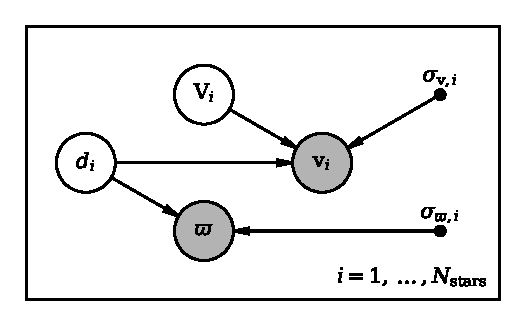
\includegraphics{figures/simple-pgm.pdf}
    \caption{Probabilistic graphical model for the simple (non-hierarchical) model. Parameters are given by circular nodes and connected by arrows showing the direction of dependency. Observed parameters are shaded, and fixed parameters are given by filled dots. The box represents a set of parameters belonging to the \(i\)-th star.}
    \label{fig:simple-pgm}
\end{figure}

In Figure \ref{fig:simple-pgm}, we show a probabilistic graphical model of the simple model. This shows the connections between parameters in the model. There is no hierarchy in this model because each parameter exists within the box, meaning no information is shared between stars. However, we know that the stellar distances are correlated. For example, it is highly unlikely that one star in the cluster is at a distance of 5 and another is at a distance of 15. If we can exploit this expectation, we could improve our prior and thus improve the inference of \(d_i\) and \(\absmag_i\).

\subsection{Hierarchical model}

In this section, we present a hierarchical Bayesian model (HBM) which includes the known correlation between distances to the stars in this open cluster analogue. We assumed the stars are all members of the same open cluster. Therefore, their distances can be modelled by some distribution. For this example, we assumed that each distance is drawn from a normal distribution characterised by new \emph{hyperparameters} \(\mu_d\) and \(\sigma_d\),
%
\begin{equation}
    d_i \sim \mathcal{N}(\mu_d, \sigma_d^2).
\end{equation}
%
The hyperparameters are so-called because they take a single value for the population of stars. Hence, the hierarchy of the model arises as some parameters represent a population of stars, while others represent the individual stars in the population.

Each stellar distance, \(d_i\), is no longer independent. Hence, we modified the posterior probability distribution to account for this new correlation,
%
\begin{equation}
    p(\mu_d, \sigma_d, \vect{d}, \vect{\absmag} \mid \vect{\varpi}, \vect{\appmag}) \propto p(\vect{\varpi}, \vect{\appmag} \mid \vect{d}, \vect{\absmag}) \, p(\vect{d} \mid \mu_d, \sigma_d) \, p(\mu_d, \sigma_d, \vect{\absmag}),
\end{equation}
%
where \(p(\vect{\varpi}, \vect{\appmag} \mid \vect{d}, \vect{\absmag})\) is the likelihood --- a product over Equation \ref{eq:hbm-like},
%
\begin{equation}
    p(\vect{\varpi}, \vect{\appmag} \mid \vect{d}, \vect{\absmag}) = \prod_{i=1}^{N_\mathrm{stars}} p(\varpi_i, \appmag_i \mid d_i, \absmag_i).
\end{equation}
%
Our posterior now depends on all stars in the population, so we used a bold typeface to represent the set of individual stellar parameters. For example, \(\vect{d} \equiv d_1, \dots, d_{N_\mathrm{stars}}\).

We modelled \(d_i\) as a random variable which depends on the hyperparameters. This means our prior is now the product of a conditional distribution, \(p(\vect{d} \,|\, \mu_d, \sigma_d)\) and a prior on the remaining independent parameters, \(p(\mu_d, \sigma_d, \vect{\absmag})\). We write the conditional distribution for distance as a product of normal distributions,
%
\begin{equation}
    p(\vect{d} \mid \mu_d, \sigma_d) = \prod_{i=1}^{N_\mathrm{stars}} \mathcal{N}(d_i \mid \mu_d, \sigma_d^2),
\end{equation}
%
where the prior probability distribution for \(\mu_d\) and \(\sigma_d\) is,
%
\begin{equation}
    p(\mu_d, \sigma_d) = \mathcal{U}(\mu_d \mid 0, 20) \, \mathcal{N}(\ln\sigma_d \mid - \ln 10, 1).
\end{equation}
%
We chose to use a log-normal prior for \(\sigma_d\) to ensure that the parameter is positive. The standard deviation of the prior on \(\sigma_d\) approximately corresponds to a fractional uncertainty of 100 per cent. Finally, we inherited the prior on \(\absmag_i\) from the simple model.

\begin{figure}[tb]
    \centering
    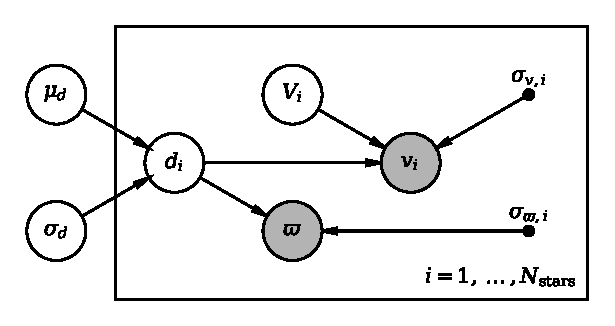
\includegraphics{figures/hbm-pgm.pdf}
    \caption{Probabilistic graphical model extension of Figure \ref{fig:simple-pgm} but for the HBM. The hyperparameters exist outside of the box to show that they govern the population of stars.}
    \label{fig:hbm-pgm}
\end{figure}

We show the probabilistic graphical model of the HBM in Figure \ref{fig:hbm-pgm}. Here, we show how all individual stellar parameters depend on \(\mu_d\) and \(\sigma_d\). We can imagine extending this framework to multiple levels, or adding additionally hyperparameters.

\subsection{Inferring the model parameters}

To infer the model parameters, we need to calculate the marginalised posterior distributions for each parameter. We could obtain this analytically by integrating the full posterior distribution over all model parameters except for the parameter of interest. Alternatively, we can approximate the marginalised posterior using a Markov Chain Monte Carlo (MCMC) sampling algorithm. We chose the latter approach because it is scalable to more complicated models where the marginalisation is not analytically solvable.

We used the No U-Turn Sampler \citep[NUTS;][]{Hoffman.Gelman2014} as implemented in the \textsc{NumPyro} Python package \citep{Phan.Pradhan.ea2019,Bingham.Chen.ea2019} to sample from the approximate posterior distribution for both models. We took 1500 samples, with the first 500 samples discarded as `warmup' steps, repeated over 10 MCMC chains. For the HBM, we increased the target accept probability from 0.8 to 0.98, to minimise the number of divergences encountered during sampling. The resulting marginalised posterior samples amounted to \num{10000} per parameter.

\subsection{Comparing the models}

\begin{figure}[p]
    \centering
    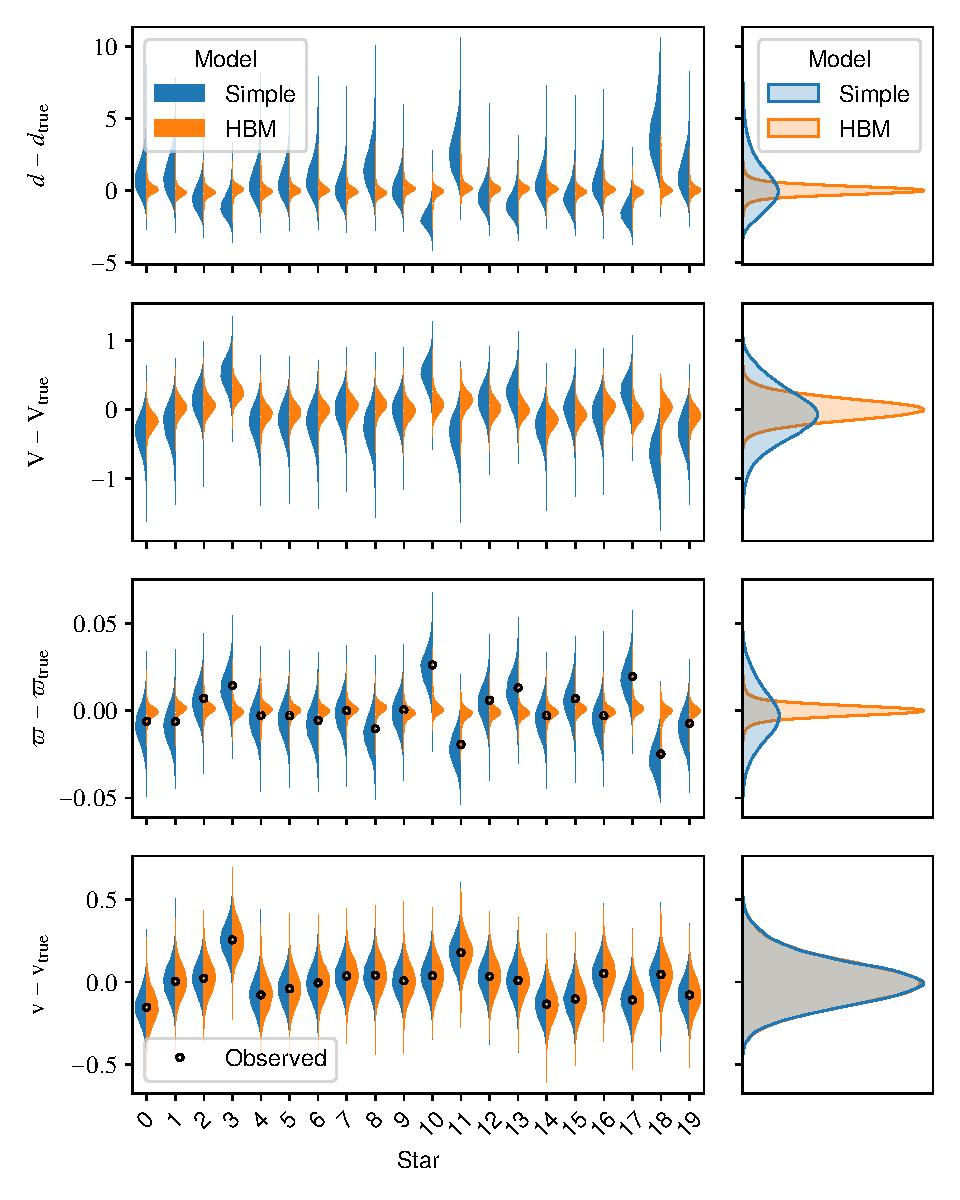
\includegraphics{figures/hbm-results.pdf}
    \caption{Plots comparing the simple model (\emph{blue}) to the HBM (\emph{orange}). \emph{Left column:} Split violin-plots showing the difference between marginalised posterior distributions for the parameters and their true values. \emph{Right column:} Kernel density estimates of the parameter-truth differences over all \(N_\mathrm{stars}\). Observed values of the parameters are given by empty black circles.}
    \label{fig:hbm-results}
\end{figure}

We compared the difference between model parameters and their true values in Figure \ref{fig:hbm-results}. The HBM showed clear improvement over the simple model in all parameters except for \(\appmag\). Pooling the distances shrank their standard deviations by about one third and converged on their true values. This had the effect of removing the observational noise on \(\varpi\), as we can see the posterior predictions for parallax also converged on their true values. Since \(\appmag\) depends on both \(d\) and \(\absmag\), improved distances also improved the absolute magnitudes.

\todo{Hand-wavy why apparent magnitude saw no improvement was because the observational noise on parallax had a larger impact on the distance than with apparent magnitude. \(\appmag \propto \log_{10}d\), whereas \(\varpi = d^{-1}\). Additionally, the fractional uncertainty on parallax was greater than that of apparent magnitude. The noise budget is dominated by the parallax, so this is the first to be improved by better distances. \(\sigma_\varpi/\varpi = \sigma_d \varpi\), but \(\sigma_\appmag / \appmag \propto \sigma_d \varpi / \appmag\)}

\begin{figure}[tb]
    \centering
    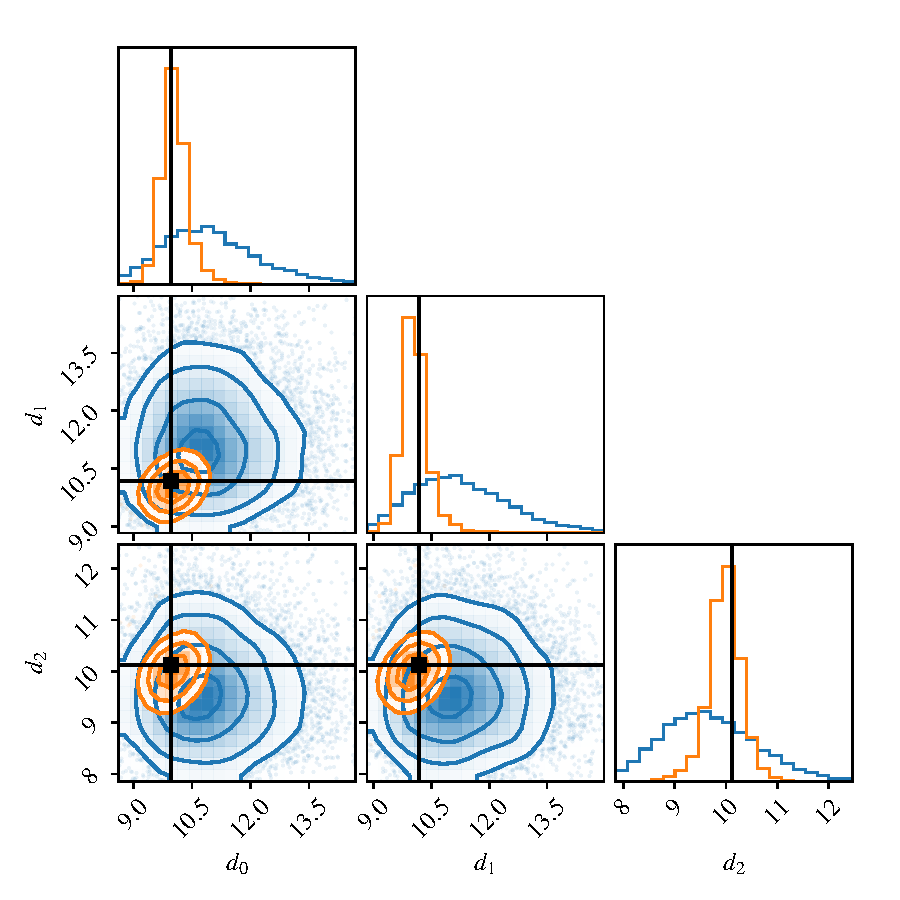
\includegraphics{figures/hbm-dist-corr.pdf}
    \caption{A corner plot showing the marginalised and joint posterior distributions of the distance to the first three stars. The simple model is shown in \emph{blue} and the HMB is shown in \emph{orange}. The true values are given by the \emph{black} lines. The range of the distributions are limited to 98 per cent of the simple model's marginalised posteriors.}
    \label{fig:hbm-corr}
\end{figure}

In Figure \ref{fig:hbm-corr}, we compared the joint and marginalised posteriors of the distance to a few of the stars. The HBM found distances to higher precision, with typical standard deviations of \(s_{d,i} \approx 0.35\) compared to \(s_{d,i} \approx 1.2\) from the simple model. We also noticed a one-to-one correlation between \(d\) present in the HBM but not in the simple model. This was a result of the correlation introduction by the population-prior on \(d\). For each distance, we saw how a lower value in one corresponded to a lower value for the others. This represents our belief that cluster members should share a similar distance. On the other hand, the simple model suggested it was, for example, just as likely to find one star at a distance of 9 and another at 12 as it would be for both to be at a distance of 11.

\begin{figure}[tb]
    \centering
    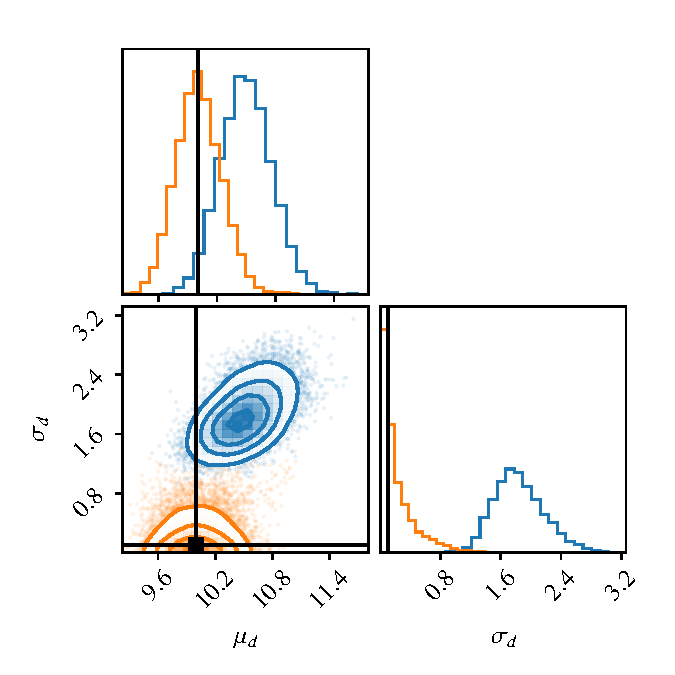
\includegraphics{figures/hbm-global.pdf}
    \caption{The joint and marginalised posterior distributions for the mean (\(\mu_d\)) and standard deviation (\(\sigma_d\)) of stellar distances in the cluster. The simple model is shown in \emph{blue} and the HMB is shown in \emph{orange}. The true values are given by the \emph{black} lines.}
    \label{fig:hbm-global}
\end{figure}

One consequence of the HBM was that it parametrised the population mean (\(\mu_d\)) and standard deviation (\(\sigma_d\)) of the distances to stars in the cluster independently from the observed noise. For the simple model, we estimated \(\mu_d\) and \(\sigma_d\) by taking the sample mean and standard deviation of distances in the cluster for each posterior sample. We compared the resulting posterior distributions for \(\mu_d\) and \(\sigma_d\) from the two models in Figure \ref{fig:hbm-global}. We found the mean distance from the simple model was \(\mu_d = 10.50 \pm 0.27\), whereas the HBM was more accurate with \(\mu_d = 10.01 \pm 0.24\). We also found the simple model massively overestimated the standard deviation of cluster distances with \(\sigma_d = 1.815_{-0.293}^{+0.360}\), compared to the HBM's more accurate value of \(\sigma_d = 0.131_{-0.088}^{+0.280}\). The simple model cannot easily distinguish between the uncertainty on individual distances and the spread of the population.

\subsection{Scaling with the number of stars}

To test how the model scales with number of stars, we repeated the HBM method for different \(N_\mathrm{stars}\). We randomly generated true and observed parameters in the same way as described at the beginning of \ref{sec:hbm-dist} for 320 stars. The observables were different to the last section, but drawn from the same distributions. We then sampled from the HBM for the first 20, 80 and 320 stars. These represented ratios in \(N_\mathrm{stars}^{1/2}\) of \(1\), \(1/2\) and \(1/4\) respectively.

\begin{figure}[tb]
    \centering
    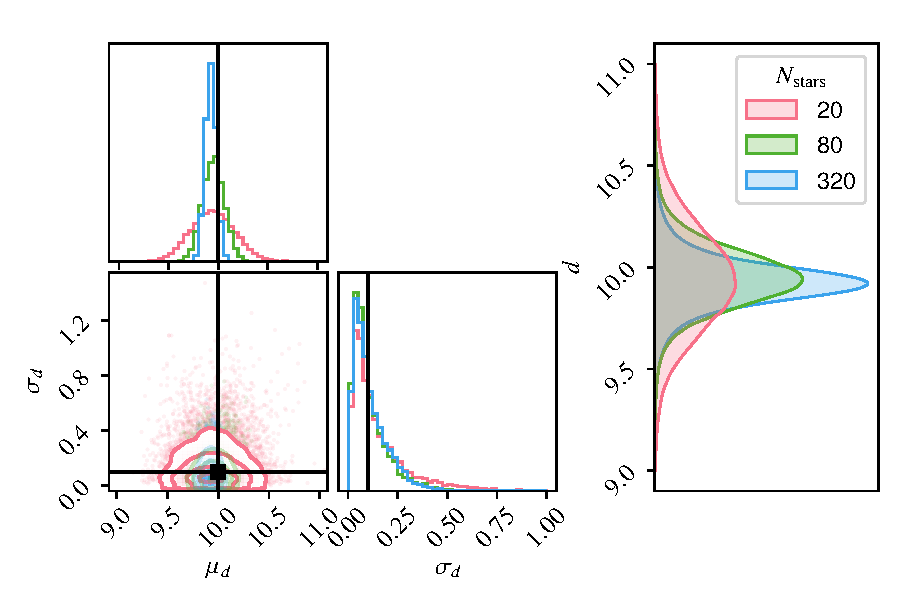
\includegraphics{figures/hbm-extended.pdf}
    \caption{Joint and marginalised posterior distributions from the HBM for 20, 80 and 320 stars.}
    \label{fig:hbm-extended}
\end{figure}

Figure \ref{fig:hbm-extended} shows how the distance estimates improved with increasing number of stars observed, \(N_\mathrm{stars}=(20,80,320)\). Unsurprisingly, the standard deviation on \(\mu_d\) decreased by a factor of \(N_\mathrm{stars}^{1/2}\) each time, with \(s_{\mu_d} \approx (0.24, 0.12, 0.06)\). We also expected a similar reduction in uncertainty for individual distances, albeit limited by the observational noise. Typical standard deviations for \(d_i\) were \(s_{d,i} \approx (0.30, 0.17, 0.15)\). We found the distance uncertainties halved from \(20\) to \(80\) stars, but this effect lessened with 320 stars. This demonstrated the value of an HBM in getting the most out a limited number of noisy observations.

\section[Stellar inference]{Inferring stellar parameters}

Typically, we model stars independently of each other. However, there a several factors which could correlate from star-to-star. \todo{Introduce the idea of hierarchically modelling stars. Finish by explaining that this is slow and difficult to do ad hoc, e.g. propose initial parameters from population distribution and evolve a model. We would like a way to emulate MESA etc. This leads to the next section on emulating stellar models with machine learning.}
